\section{Validazione e Collaudo}
\textit{Dal 2021-04-09 al 2021-05-10}


\begin{figure}[H]
	\centering
	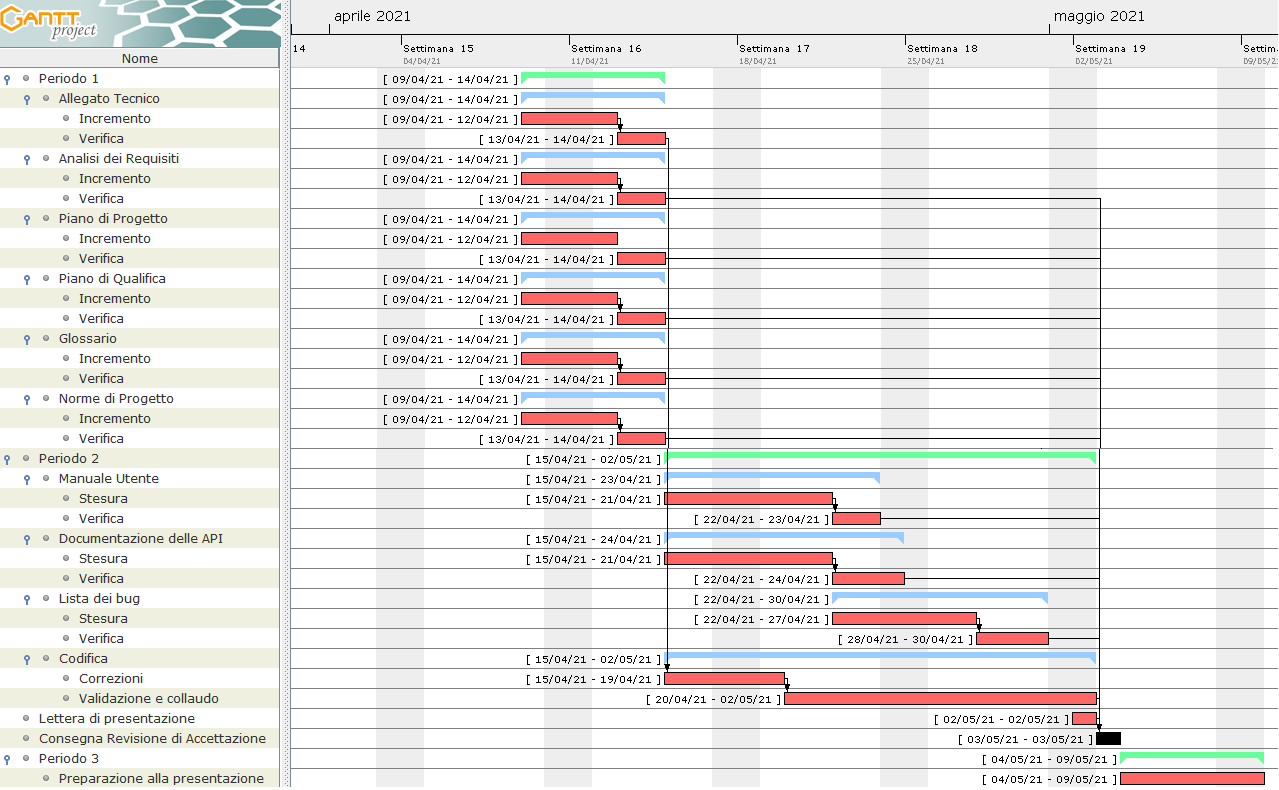
\includegraphics[scale=0.45]{res/images/gantt_fase/06_gantt_validazione}
	\caption{Diagramma di Gantt\textsubscript{G} relativo alla Validazione e Collaudo}
\end{figure}


\subsection{Periodo 1}

\subsubsection{Pianificazione preventiva}

\paragraph{Attività}
\subparagraph*{}

\planningTable{
	Incremento Analisi dei Requisiti & L'avanzamento nello sviluppo del prodotto chiarirà alcuni aspetti che nella fase\textsubscript{G} di Analisi risultavano oscuri, e potrebbe evidenziare delle criticità non inizialmente considerate. Se necessario, viene raffinata l'\textsc{Analisi dei Requisiti} &  & Verificatore
\tabularnewline 
Incremento Piano di Progetto & Il \textsc{Piano di Progetto} viene migliorato fornendo maggior dettaglio, oltre che integrato con il consuntivo del periodo trascorso &  & Responsabile
\tabularnewline 
Incremento Glossario & Viene integrato con nuovi termini &  & Responsabile
\tabularnewline 
Incremento Piano di Qualifica & Il cruscotto viene aggiornato con i dati rilevati sul periodo trascorso &  & Responsabile
\tabularnewline 
\caption{Pianificazione preventiva - Validazione e Collaudo - Periodo 1}
}

\paragraph{Preventivo}
\subparagraph*{}

\hspace{-1cm}
\begin{minipage}{.50\textwidth}
\smallPreventivoTable{
	Responsabile & 2 & 60\\ 
Verificatore & 4 & 60\\ 
Analista & 4 & 100\\ 
Amministratore & 0 & 0\\ 
Programmatore & 0 & 0\\ 
Progettista & 0 & 0\\ 
\hlinetable 
\textbf{Totale} & \textbf{10} & \textbf{220}\\ 
\end{tabular} 
\caption{Preventivo - Validazione e Collaudo - Periodo 1}
}
\end{minipage}
\hspace{1cm}
\begin{minipage}{.40\textwidth}
\begin{figure}[H]
	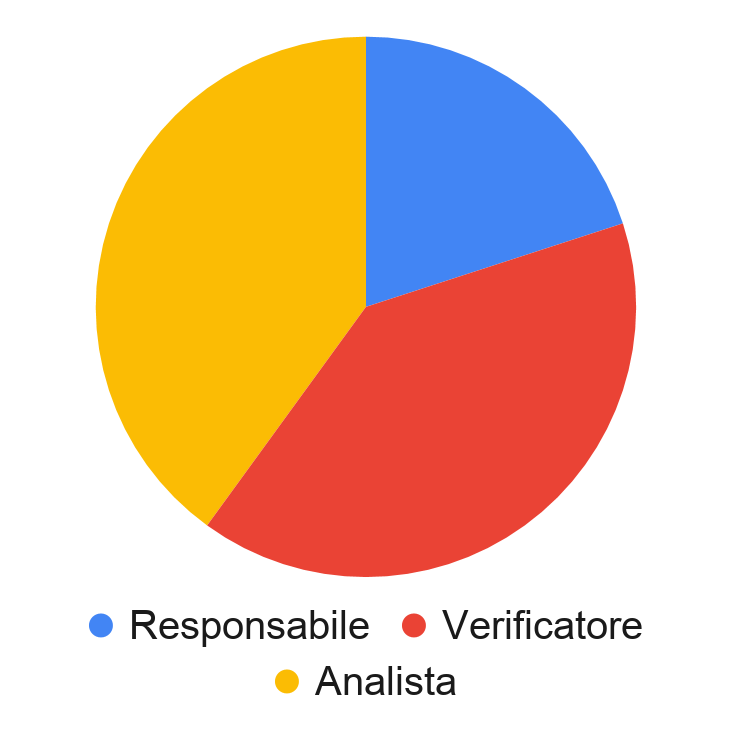
\includegraphics[scale=0.21]{res/images/charts/preventivo_priori/Grafico4-9.png}
	\caption{Distribuzione dei costi: preventivo - Validazione e Collaudo - Periodo 1}
\end{figure}
\end{minipage} 





\subsubsection{Pianificazione di periodo}


\begin{figure}[H]
	\centering
	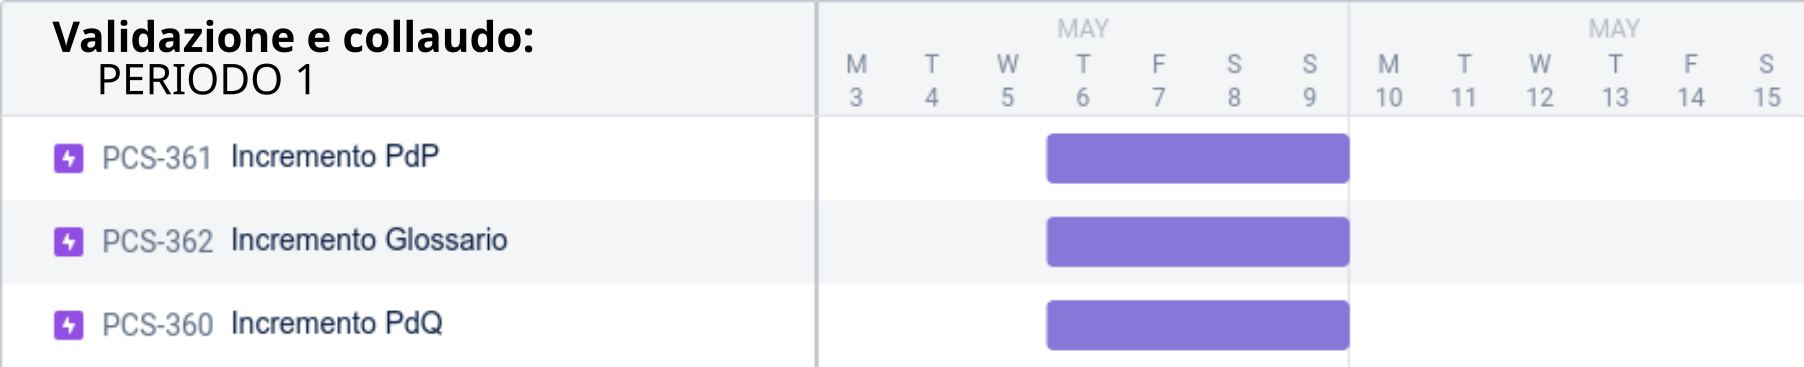
\includegraphics[scale=0.55]{res/images/gantt_periodo/valid_1_gantt.png}
	\caption{Gantt di periodo\textsubscript{G} - Validazione e Collaudo - Periodo 1}
\end{figure}

\paragraph{Attività}
\subparagraph*{}

\planningTable{
	Incremento Piano di Progetto & Il \textsc{Piano di Progetto} viene integrato con il consuntivo del periodo trascorso. & 1 & Responsabile
\tabularnewline 
Incremento Glossario & Viene integrato con nuovi termini. & 1 & Responsabile
\tabularnewline 
Incremento Piano di Qualifica & Il cruscotto viene aggiornato con i dati rilevati sul periodo trascorso, in particolare sui test effettuati. & 4 & Verificatore
\tabularnewline 
\caption{Pianificazione di periodo - Validazione e Collaudo - Periodo 1}
}



\paragraph{Preventivo orario ed economico}
\subparagraph*{}

\contabilitaTable{
	Chiarello Sofia & 0 & 0 & 0 & 0 & 0 & 0 & \textbf{0}\\ 
Crivellari Alberto & 0 & 4 & 0 & 0 & 0 & 0 & \textbf{4}\\ 
De Renzis Simone & 1 & 0 & 0 & 0 & 0 & 0 & \textbf{1}\\ 
Greggio Nicolò & 1 & 0 & 0 & 0 & 0 & 0 & \textbf{1}\\ 
Tessari Andrea & 0 & 0 & 0 & 0 & 0 & 0 & \textbf{0}\\ 
Zuccolo Giada & 0 & 0 & 0 & 0 & 0 & 0 & \textbf{0}\\ 
\hlinetable 
\textbf{Totale orario} & \textbf{2} & \textbf{4} & \textbf{0} & \textbf{0} & \textbf{0} & \textbf{0} & \textbf{6}\\ 
\textbf{Totale costo} & \textbf{60} & \textbf{60} & \textbf{0} & \textbf{0} & \textbf{0} & \textbf{0} & \textbf{120}\\ 
\end{tabular} 
\caption{Preventivo di periodo\textsubscript{G} - Validazione e Collaudo - Periodo 1}
}

\begin{figure}[H]
	\centering
	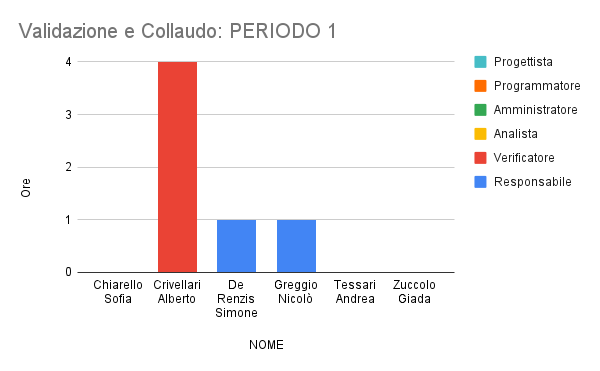
\includegraphics[scale=0.6]{res/images/charts/preventivo/valid_1.png}
	\caption{Distribuzione oraria per componente: preventivo di periodo\textsubscript{G} - Validazione e Collaudo - Periodo 1}
\end{figure}



\subsubsection{Riscontro di fine periodo}


\paragraph{Consuntivo orario ed economico}
\subparagraph*{}

\contabilitaTable{
	Chiarello Sofia & 0 & 0 & 0 & 0 & 0 & 0 & \textbf{0} \\ 
Crivellari Alberto & 0 & 4 & 0 & 0 & 0 & 0 & \textbf{4} \\ 
De Renzis Simone & 1 & 0 & 0 & 0 & 0 & 0 & \textbf{1} \\ 
Greggio Nicolò & 1 & 0 & 0 & 0 & 0 & 0 & \textbf{1} \\ 
Tessari Andrea & 0 & 0 & 0 & 0 & 0 & 0 & \textbf{0} \\ 
Zuccolo Giada & 0 & 0 & 0 & 0 & 0 & 0 & \textbf{0} \\ 
\hlinetable 
\textbf{Totale orario} & \textbf{2} & \textbf{4} & \textbf{0} & \textbf{0} & \textbf{0} & \textbf{0} & \textbf{6} \\ 
\textbf{Differenza orario} & \textbf{0} & \textbf{0} & \textbf{0} & \textbf{0} & \textbf{0} & \textbf{0} & \textbf{0} \\ 
\textbf{Totale costi} & \textbf{60} & \textbf{60} & \textbf{0} & \textbf{0} & \textbf{0} & \textbf{0} & \textbf{120} \\ 
\textbf{Differenza costi} & \textbf{0} & \textbf{0} & \textbf{0} & \textbf{0} & \textbf{0} & \textbf{0} & \textbf{0} \\ 
\end{tabular} 
\caption{Consuntivo - Validazione e Collaudo - Periodo 1}
}

\begin{figure}[H]
	\centering
	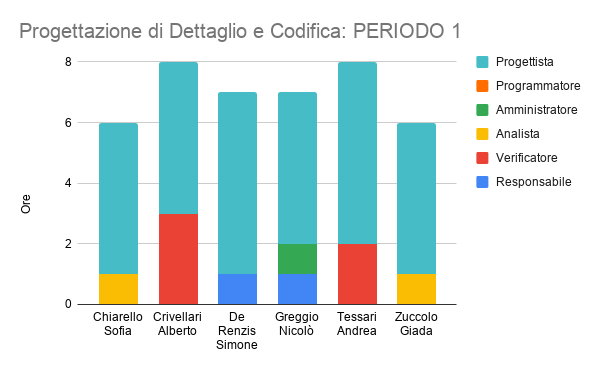
\includegraphics[scale=0.6]{res/images/charts/consuntivo/prog_dett_1.png}
	\caption{Distribuzione oraria per componente: consuntivo - Validazione e Collaudo - Periodo 1}
\end{figure}


Il periodo\textsubscript{G} chiude in \textbf{********************} *****************************


\paragraph{Preventivo a finire}
\subparagraph*{}

\pafTable{
	Avvio & 1 & Consuntivo & 1060
\tabularnewline
Analisi dei Requisiti & 1 & Consuntivo & 3380
\tabularnewline
Analisi dei Requisiti & 2 & Consuntivo & 255
\tabularnewline
Progettazione Architetturale & 1 & Consuntivo & 2220
\tabularnewline
Progettazione Architetturale & 2 & Consuntivo & 2000
\tabularnewline
Progettazione Architetturale & 3 & Consuntivo & 150
\tabularnewline
Progettazione di Dettaglio e Codifica & 1 & Consuntivo & 909
\tabularnewline
Progettazione di Dettaglio e Codifica & 2 & Consuntivo & 2760
\tabularnewline
Progettazione di Dettaglio e Codifica & 3 & Consuntivo & 388
\tabularnewline
Validazione e Collaudo & 1 & Consuntivo & 120
\tabularnewline
Validazione e Collaudo & 2 & Preventivo di periodo\textsubscript{G} & 2130
\tabularnewline
Validazione e Collaudo & 3 & Preventivo & 60
\tabularnewline
\textbf{Totale} & \textbf{} & \textbf{} & \textbf{15432}
\tabularnewline
\textbf{Totale rendicontato} & \textbf{} & \textbf{} & \textbf{10737}
\tabularnewline
\caption{Preventivo a finire - Validazione e Collaudo - Periodo 1}
}

******************************************************





\pagebreak
\subsection{Periodo 2}

\subsubsection{Pianificazione preventiva}

\paragraph{Attività}
\subparagraph*{}

\planningTable{
	Validazione e Collaudo & vengono eseguiti ulteriori test per consolidare e garantire la qualità del prodotto. Il \textsc{Piano di Qualifica} è il documento di riferimento per quest'attività. &  & Verificatore
\tabularnewline 
Manuale Utente & Il \textsc{Manuale Utente} specifica le modalità d'uso del software agli utenti utilizzatori &  & Progettista
\tabularnewline 
Documentazione delle API & Come richiesto dal proponente, la documentazione conterrà le API di comunicazione tra server e unità &  & Progettista
\tabularnewline 
Lista dei bug & Come richiesto dal proponente, la documentazione conterrà i bug riscontrati durante lo sviluppo del software &  & Progettista
\tabularnewline 
\caption{Pianificazione preventiva - Validazione e Collaudo - Periodo 2}
}

\paragraph{Preventivo}
\subparagraph*{}

\hspace{-1cm}
\begin{minipage}{.50\textwidth}
\smallPreventivoTable{
	Responsabile & 0 & 0\\ 
Verificatore & 90 & 1350\\ 
Analista & 0 & 0\\ 
Amministratore & 0 & 0\\ 
Programmatore & 31 & 465\\ 
Progettista & 15 & 330\\ 
\hlinetable 
\textbf{Totale} & \textbf{136} & \textbf{2145}\\ 
\end{tabular} 
\caption{Preventivo - Validazione e Collaudo - Periodo 2}
}
\end{minipage}
\hspace{1cm}
\begin{minipage}{.40\textwidth}
\begin{figure}[H]
	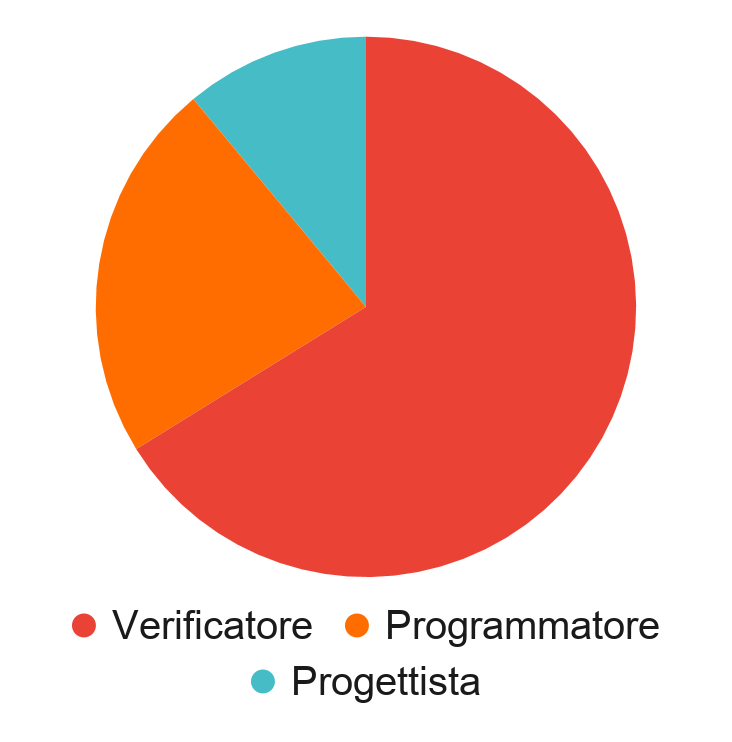
\includegraphics[scale=0.21]{res/images/charts/preventivo_priori/Grafico4-10.png}
	\caption{Distribuzione dei costi: preventivo - Validazione e Collaudo - Periodo 2}
\end{figure}
\end{minipage} 




\subsubsection{Pianificazione di periodo}


\begin{figure}[H]
	\centering
	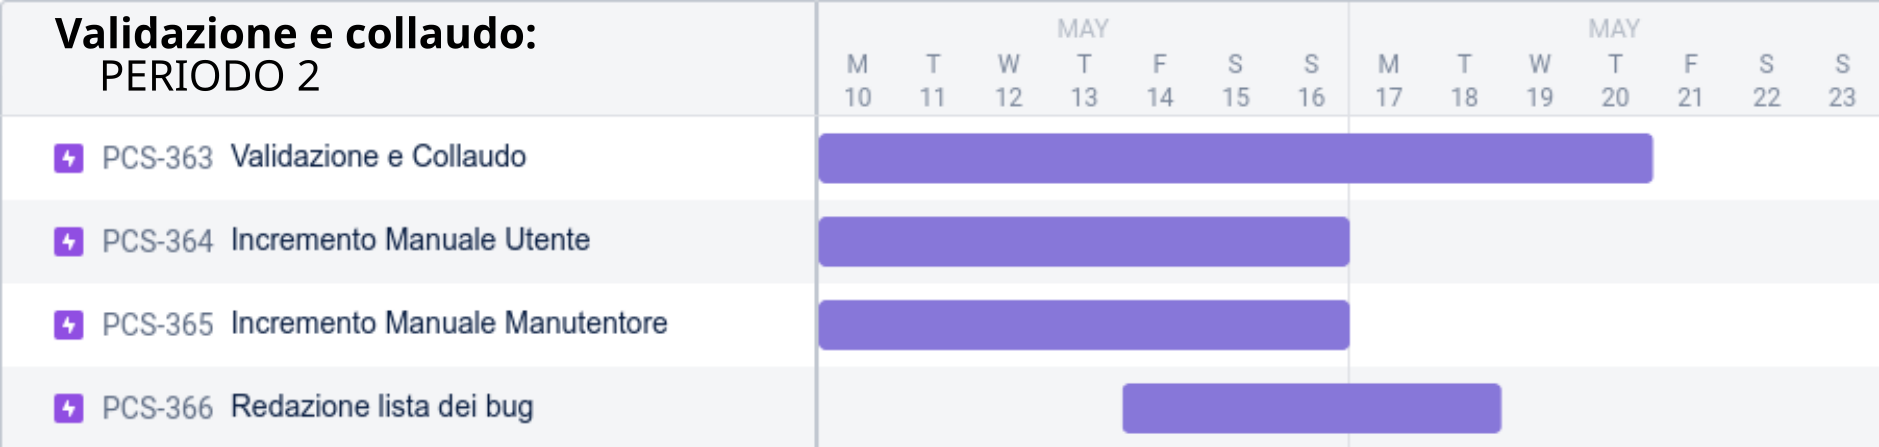
\includegraphics[scale=0.55]{res/images/gantt_periodo/valid_2_gantt.png}
	\caption{Gantt di periodo\textsubscript{G} - Validazione e Collaudo - Periodo 2}
\end{figure}

\paragraph{Attività}
\subparagraph*{}

\planningTable{
	Validazione e Collaudo & Vengono ultimati i test di unità, realizzati i test di integrazione e di sistema per certificare la qualità del prodotto. Il \textsc{Piano di Qualifica} è il documento di riferimento per quest'attività. & 121 & Verificatore, Programmatore
\tabularnewline 
Incremento Manuale Utente & Il \textsc{Manuale Utente} viene integrato presentando anche le ultime ottimizzazioni nelle funzionalità e nell'intefaccia. & 8 & Progettista
\tabularnewline 
Incremento Manuale Manutentore & Viene incremenentato il \textsc{Manuale Manutentore} per integrare e dettagliare le eventuali minori modifiche nell'architettura del software. In questo documento confluisce la documentazione del prodocollo di comunicazione attuato, come da requisiti del proponente. & 5 & Progettista
\tabularnewline 
Lista dei bug\textsubscript{G} & Come richiesto dal proponente, la documentazione conterrà i bug\textsubscript{G} riscontrati durante lo sviluppo del software. & 2 & Progettista
\tabularnewline 
\caption{Pianificazione di periodo\textsubscript{G} - Validazione e Collaudo - Periodo 2}
}



\paragraph{Preventivo orario ed economico}
\subparagraph*{}

\contabilitaTable{
	Chiarello Sofia & 0 & 10 & 0 & 0 & 9 & 4 & \textbf{23}\\ 
Crivellari Alberto & 0 & 20 & 0 & 0 & 1 & 0 & \textbf{21}\\ 
De Renzis Simone & 0 & 10 & 0 & 0 & 10 & 1 & \textbf{21}\\ 
Greggio Nicolò & 0 & 10 & 0 & 0 & 10 & 2 & \textbf{22}\\ 
Tessari Andrea & 0 & 10 & 0 & 0 & 10 & 4 & \textbf{24}\\ 
Zuccolo Giada & 0 & 10 & 0 & 0 & 10 & 4 & \textbf{24}\\ 
\hlinetable 
\textbf{Totale orario} & \textbf{0} & \textbf{70} & \textbf{0} & \textbf{0} & \textbf{50} & \textbf{15} & \textbf{135}\\ 
\textbf{Totale costo} & \textbf{0} & \textbf{1050} & \textbf{0} & \textbf{0} & \textbf{750} & \textbf{330} & \textbf{2130}\\ 
\end{tabular} 
\caption{Preventivo di periodo\textsubscript{G} - Validazione e Collaudo - Periodo 2}
}

\begin{figure}[H]
	\centering
	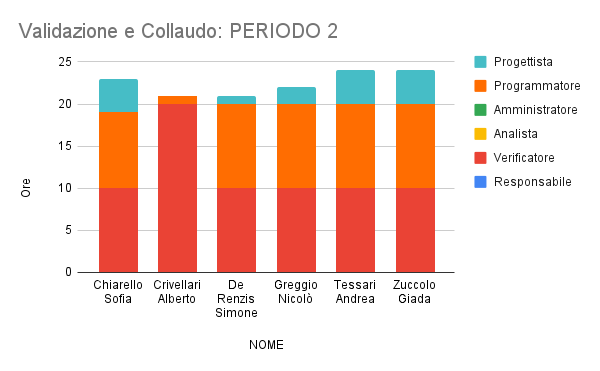
\includegraphics[scale=0.6]{res/images/charts/preventivo/valid_2.png}
	\caption{Distribuzione oraria per componente: preventivo di periodo\textsubscript{G} - Validazione e Collaudo - Periodo 2}
\end{figure}



\subsubsection{Riscontro di fine periodo}


\paragraph{Consuntivo orario ed economico}
\subparagraph*{}

\contabilitaTable{
	Chiarello Sofia & 0 & 8 & 0 & 0 & 4 & 4 & \textbf{16} \\ 
Crivellari Alberto & 0 & 14 & 0 & 0 & 0 & 0 & \textbf{14} \\ 
De Renzis Simone & 0 & 9 & 0 & 0 & 4 & 1 & \textbf{14} \\ 
Greggio Nicolò & 0 & 8 & 0 & 0 & 4 & 2 & \textbf{14} \\ 
Tessari Andrea & 0 & 9 & 0 & 0 & 4 & 4 & \textbf{17} \\ 
Zuccolo Giada & 0 & 9 & 0 & 0 & 4 & 4 & \textbf{17} \\ 
\hlinetable 
\textbf{Totale orario} & \textbf{0} & \textbf{57} & \textbf{0} & \textbf{0} & \textbf{20} & \textbf{15} & \textbf{92} \\ 
\textbf{Differenza orario} & \textbf{0} & \textbf{-13} & \textbf{0} & \textbf{0} & \textbf{-30} & \textbf{0} & \textbf{-43} \\ 
\textbf{Totale costi} & \textbf{0} & \textbf{855} & \textbf{0} & \textbf{0} & \textbf{300} & \textbf{330} & \textbf{1485} \\ 
\textbf{Differenza costi} & \textbf{0} & \textbf{-195} & \textbf{0} & \textbf{0} & \textbf{-450} & \textbf{0} & \textbf{-645} \\ 
\end{tabular} 
\caption{Consuntivo - Validazione e Collaudo - Periodo 2}
}

\begin{figure}[H]
	\centering
	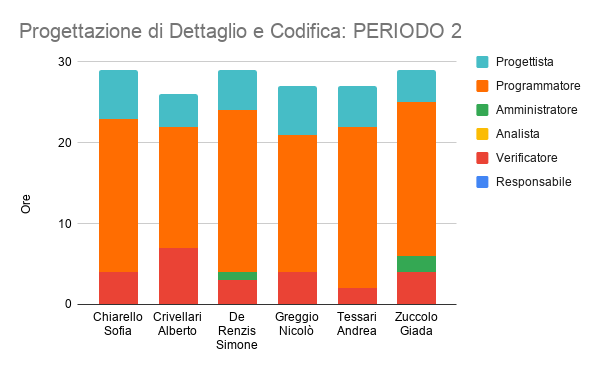
\includegraphics[scale=0.6]{res/images/charts/consuntivo/prog_dett_2.png}
	\caption{Distribuzione oraria per componente: consuntivo - Validazione e Collaudo - Periodo 2}
\end{figure}


Il periodo\textsubscript{G} chiude in \textbf{********************} *****************************


\paragraph{Preventivo a finire}
\subparagraph*{}

\pafTable{
	Avvio & 1 & Consuntivo & 1060
\tabularnewline
Analisi dei Requisiti & 1 & Consuntivo & 3380
\tabularnewline
Analisi dei Requisiti & 2 & Consuntivo & 255
\tabularnewline
Progettazione Architetturale & 1 & Consuntivo & 2220
\tabularnewline
Progettazione Architetturale & 2 & Consuntivo & 2000
\tabularnewline
Progettazione Architetturale & 3 & Consuntivo & 150
\tabularnewline
Progettazione di Dettaglio e Codifica & 1 & Consuntivo & 909
\tabularnewline
Progettazione di Dettaglio e Codifica & 2 & Consuntivo & 2760
\tabularnewline
Progettazione di Dettaglio e Codifica & 3 & Consuntivo & 388
\tabularnewline
Validazione e Collaudo & 1 & Consuntivo & 120
\tabularnewline
Validazione e Collaudo & 2 & Consuntivo & 1485
\tabularnewline
Validazione e Collaudo & 3 & Preventivo di periodo & 120
\tabularnewline
\textbf{Totale} & \textbf{} & \textbf{} & \textbf{14847}
\tabularnewline
\textbf{Totale rendicontato} & \textbf{} & \textbf{} & \textbf{10152}
\tabularnewline
\caption{Preventivo a finire - Validazione e Collaudo - Periodo 2}
}

******************************************************





\pagebreak
\subsection{Periodo 3}

\subsubsection{Pianificazione preventiva}

\paragraph{Attività}
\subparagraph*{}

\planningTable{
	Preparazione alla presentazione & Viene preparato il materiale necessario alla presentazione & 3 & Amministratore
\tabularnewline 
\caption{Pianificazione preventiva - Validazione e Collaudo - Periodo 3}
}

\paragraph{Preventivo}
\subparagraph*{}


\hspace{-1cm}
\begin{minipage}{.50\textwidth}
\smallPreventivoTable{
	Responsabile & 0 & 0\\ 
Verificatore & 0 & 0\\ 
Analista & 0 & 0\\ 
Amministratore & 3 & 60\\ 
Programmatore & 0 & 0\\ 
Progettista & 0 & 0\\ 
\hlinetable 
\textbf{Totale} & \textbf{3} & \textbf{60}\\ 
\end{tabular} 
\caption{Preventivo - Validazione e Collaudo - Periodo 3}
}
\end{minipage}
\hspace{1cm}
\begin{minipage}{.40\textwidth}
\begin{figure}[H]
	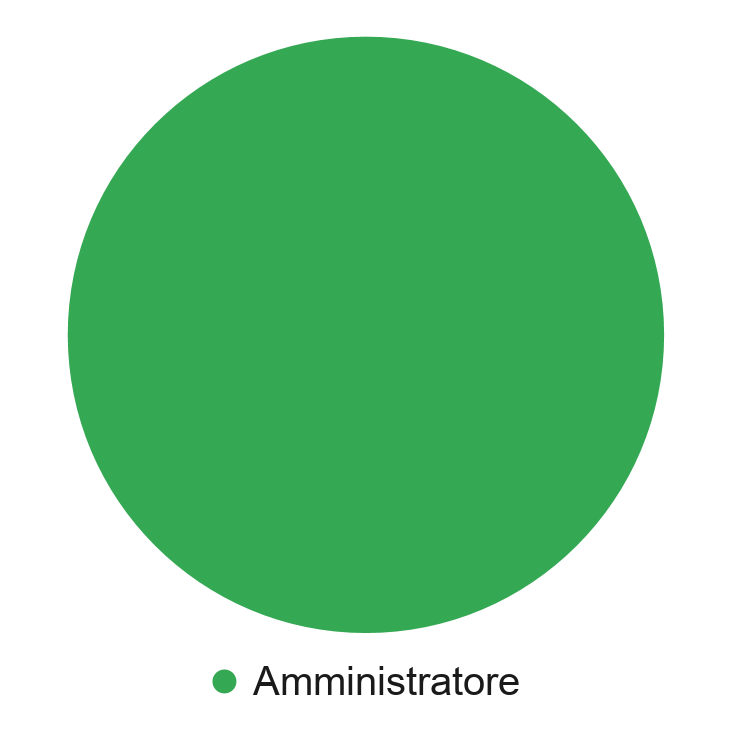
\includegraphics[scale=0.21]{res/images/charts/preventivo_priori/Grafico4-11.png}
	\caption{Distribuzione dei costi: preventivo - Validazione e Collaudo - Periodo 3}
\end{figure}
\end{minipage} 


\subsubsection{Pianificazione di periodo}


\begin{figure}[H]
	\centering
	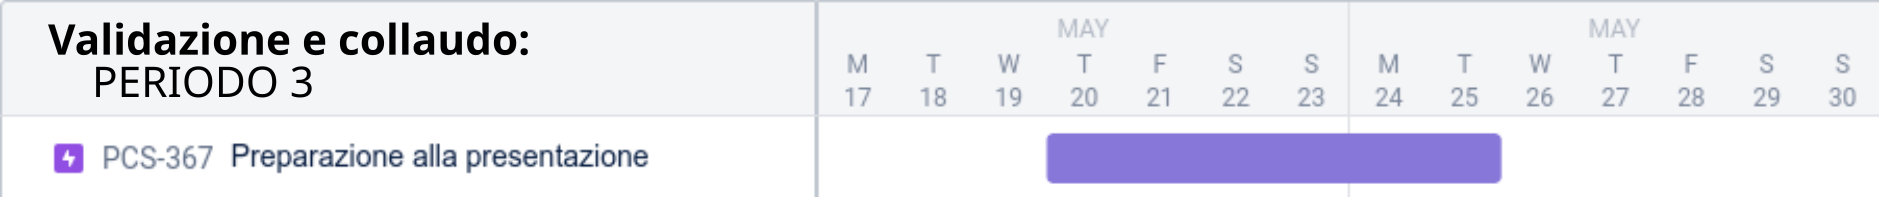
\includegraphics[scale=0.55]{res/images/gantt_periodo/valid_3_gantt.png}
	\caption{Gantt di periodo\textsubscript{G} - Validazione e Collaudo - Periodo 3}
\end{figure}

\paragraph{Attività}
\subparagraph*{}

\planningTable{
	Preparazione alla presentazione & Viene preparato il materiale necessario alla presentazione. & 3 & Amministratore
\tabularnewline 
\caption{Pianificazione di periodo\textsubscript{G} - Validazione e Collaudo - Periodo 3}
}



\paragraph{Preventivo orario ed economico}
\subparagraph*{}

\contabilitaTable{
	Chiarello Sofia & 0 & 0 & 0 & 1 & 0 & 0 & \textbf{1}\\ 
Crivellari Alberto & 0 & 0 & 0 & 2 & 0 & 0 & \textbf{2}\\ 
De Renzis Simone & 0 & 0 & 0 & 0 & 0 & 0 & \textbf{0}\\ 
Greggio Nicolò & 0 & 0 & 0 & 1 & 0 & 0 & \textbf{1}\\ 
Tessari Andrea & 0 & 0 & 0 & 1 & 0 & 0 & \textbf{1}\\ 
Zuccolo Giada & 0 & 0 & 0 & 1 & 0 & 0 & \textbf{1}\\ 
\hlinetable 
\textbf{Totale orario} & \textbf{0} & \textbf{0} & \textbf{0} & \textbf{6} & \textbf{0} & \textbf{0} & \textbf{6}\\ 
\textbf{Totale costo} & \textbf{0} & \textbf{0} & \textbf{0} & \textbf{120} & \textbf{0} & \textbf{0} & \textbf{120}\\ 
\end{tabular} 
\caption{Preventivo di periodo\textsubscript{G} - Validazione e Collaudo - Periodo 3}
}

\begin{figure}[H]
	\centering
	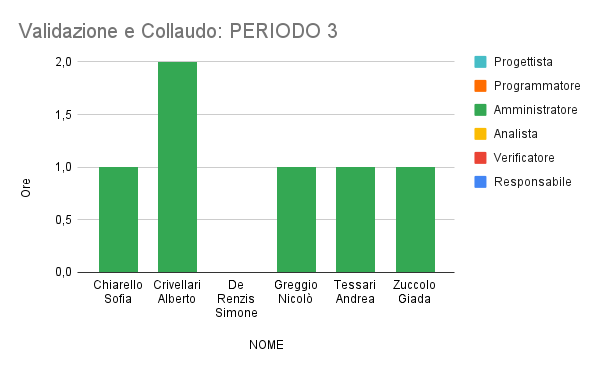
\includegraphics[scale=0.6]{res/images/charts/preventivo/valid_3.png}
	\caption{Distribuzione oraria per componente: preventivo di periodo\textsubscript{G} - Validazione e Collaudo - Periodo 3}
\end{figure}



\subsubsection{Riscontro di fine periodo}


\paragraph{Consuntivo orario ed economico}
\subparagraph*{}

\contabilitaTable{
	Chiarello Sofia & 0 & 0 & 0 & 1 & 0 & 0 & \textbf{1} \\ 
Crivellari Alberto & 0 & 0 & 0 & 2 & 0 & 0 & \textbf{2} \\ 
De Renzis Simone & 0 & 0 & 0 & 0 & 0 & 0 & \textbf{0} \\ 
Greggio Nicolò & 0 & 0 & 0 & 1 & 0 & 0 & \textbf{1} \\ 
Tessari Andrea & 0 & 0 & 0 & 1 & 0 & 0 & \textbf{1} \\ 
Zuccolo Giada & 0 & 0 & 0 & 1 & 0 & 0 & \textbf{1} \\ 
\hlinetable 
\textbf{Totale orario} & \textbf{0} & \textbf{0} & \textbf{0} & \textbf{6} & \textbf{0} & \textbf{0} & \textbf{6} \\ 
\textbf{Differenza orario} & \textbf{0} & \textbf{0} & \textbf{0} & \textbf{0} & \textbf{0} & \textbf{0} & \textbf{0} \\ 
\textbf{Totale costi} & \textbf{0} & \textbf{0} & \textbf{0} & \textbf{120} & \textbf{0} & \textbf{0} & \textbf{120} \\ 
\textbf{Differenza costi} & \textbf{0} & \textbf{0} & \textbf{0} & \textbf{0} & \textbf{0} & \textbf{0} & \textbf{0} \\ 
\end{tabular} 
\caption{Consuntivo - Validazione e Collaudo - Periodo 3}
}

\begin{figure}[H]
	\centering
	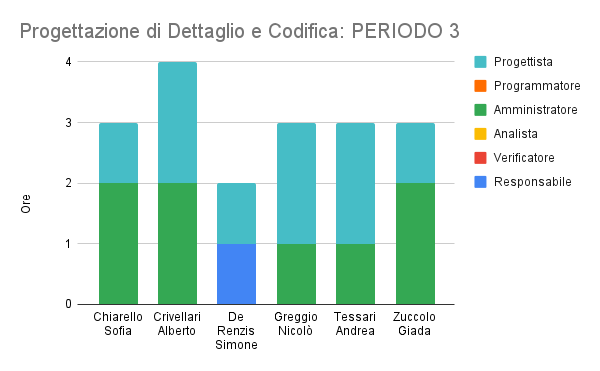
\includegraphics[scale=0.6]{res/images/charts/consuntivo/prog_dett_3.png}
	\caption{Distribuzione oraria per componente: consuntivo - Validazione e Collaudo - Periodo 3}
\end{figure}


Il periodo\textsubscript{G} chiude in \textbf{********************} *****************************


\paragraph{Preventivo a finire}
\subparagraph*{}

\pafTable{
	Avvio & 1 & Consuntivo & 1060
\tabularnewline
Analisi dei Requisiti & 1 & Consuntivo & 3380
\tabularnewline
Analisi dei Requisiti & 2 & Consuntivo & 255
\tabularnewline
Progettazione Architetturale & 1 & Consuntivo & 2220
\tabularnewline
Progettazione Architetturale & 2 & Consuntivo & 2000
\tabularnewline
Progettazione Architetturale & 3 & Consuntivo & 150
\tabularnewline
Progettazione di Dettaglio e Codifica & 1 & Consuntivo & 909
\tabularnewline
Progettazione di Dettaglio e Codifica & 2 & Consuntivo & 2760
\tabularnewline
Progettazione di Dettaglio e Codifica & 3 & Consuntivo & 388
\tabularnewline
Validazione e Collaudo & 1 & Consuntivo & 120
\tabularnewline
Validazione e Collaudo & 2 & Consuntivo & 1485
\tabularnewline
Validazione e Collaudo & 3 & Consuntivo & 120
\tabularnewline
\textbf{Totale} & \textbf{} & \textbf{} & \textbf{14847}
\tabularnewline
\textbf{Totale rendicontato} & \textbf{} & \textbf{} & \textbf{10152}
\tabularnewline
\caption{Preventivo a finire - Validazione e Collaudo - Periodo 3}
}

******************************************************
